%
% finished at Jan 22th, 2009
% Feb., 6th: add a section of spin polarized states
%            revised the introduction section by adding two items.
%            however, the writing may need to be revised.
%
% revision:
% Nov. 13th: the most important thing in this chapter is that 
% why the unrestricted determinant is not the eigen function for 
% the $S^{2}$. Now it has been made clear.
% we  simply add some illustration on the section of "general
% derivation of the spin operator" part.
% also we cut off some redundant contents so that to make the 
% description more clear. Now much satisfied. 
%
%
\chapter{Spin Operator in Quantum Chemistry}
%
% 1  introduction: consider the spin operator and symmetry operator
%               in quantum chemistry
% 2  spin operator, form and expression : Sz and S2
% 3  UHF case explanation
% 4  spin contamination and how to eliminate it by the operator
%
%

%%%%%%%%%%%%%%%%%%%%%%%%%%%%%%%%%%%%%%%%%%%%%%%%%%%%%%%%%%%%%%%%%%%%%%%%%%%%%%%%%%%%%%%%%%
\section{Introduction}\label{SIC4}
%
% 1 useful in HF, CI, MP2; constructing the wave functions
% 2 spin and symmetry operator in understanding the wave functions
%   their roles are roughly same. most importantly providing the
%   non-mixing blocks in deriving the expectation values
%   2.1  the approximated wave functions will only be the mixture
%        of same type of eigen states
%   2.2  it's proof and examples
%   2.3  the expectation value for the different wave functions with
%        different eigen states will be zero
%   2.4  more of the examples are from the transition states
%        evaluation.
%
In the quantum mechanics part, we have discussed the spin for two
non-interacting electrons system. However, since that an arbitrary
molecule is always involved with more than $2$ electrons; thus in
this chapter we are going to extend the spin discussion to the $n$
electrons system.

Unlike the other operators such as the angular momentum operator,
there's no concrete expression for the spin operator in the
non-relativistic quantum mechanics. the reason for this has been
discussed in the spin chapter in the quantum mechanics. However, the
spin phenomenon plays some vital role in the quantum chemistry. In
HF chapter, we can see that exchange effects are attributed from the
electrons have the same spin, which causes the energy different
between the singlet and triplet.

Generally in the quantum chemistry, we have to select the CSCCO and
the basis functions for the system. Through the CSCCO, and by
applying the variational process on the selected basis functions; we
can finally get the wave function, and then the properties related
to the system. Here, in quantum chemistry the Hamiltonian inside the
CSCCO can be the real Hamiltonian, or approximated Hamiltonian such
as the HF operator, the Kohn-Sham operator etc.

In this process, the spin operators, as well as the symmetry
operators; play some important and special roles. Because these
operators are all commuted with the Hamiltonian (Here we assume that
the Hamiltonian does not contain the spin effects, and the symmetry
operator; such as $C^{i}_{n}$, can always commuted with
Hamiltonian), they are all selected into the CSCCO. Physically they
actually forms some independent variables to portray the whole
system except the Hamiltonian. Such consideration is accordance with
the conclusion we give in the Schrodinger chapter.

While, how to understand the use of spin operator in quantum
chemistry, as well as the other operators such as symmetry operator?
The usage can be specified into two assertions, they are:
\begin{itemize}
  \item  For the physical quantity of $\hat{P}$ in the CSCCO, if
the result approximated wave functions give some eigen value of $p$;
then it must be only composed by the basis functions which also give
the eigen value of $p$.
  \item  For the physical quantity of $\hat{P}$ in the CSCCO, if two
resulted approximated wave functions, for example, $\Phi_{1}$ and
$\Phi_{2}$; give different eigen values of $p_{1}$ and $p_{2}$; then
for any operator $\hat{Q}$ which commuted with $\hat{P}$ the
integration of $\bra{\Phi_{1}}\hat{Q}\ket{\Phi_{2}}$ must be zero.
\end{itemize}

Now we are going to give some illustrations about the two rules
above. For the first assertion, if we use the symmetry adapted basis
functions of $\chi_{i}$ to form the HF(or DFT) molecular orbitals, for
example, such molecule belongs to $C^{2}_{v}$ group; finally it
turns out that the molecular orbitals only belong to the $A_{1}$ and
$A_{2}$ type; then such $A_{2}$ MO could only composed
by the $A_{2}$ type of AO(atomic orbitals, or more precisely; the
basis sets).

Things is same for the post HF methods. For example, in the CI method
if the second excitation state of $\Phi_{2}$ (it gives the energy of
$E_{2}$ with the sequence that $E_{0} < E_{1} < E_{2}$) has the
relation that:
\begin{align}\label{}
\hat{S}^{2}\Phi_{2} &= 1(1+1) = 2 \nonumber \\
\hat{S}_{z}\Phi_{2} &= 0
\end{align}
Then the $\Phi_{2}$ could be only composed by the Slater determinants
which give the same eigen values for the $\hat{S}^{2}$ and
$\hat{S}_{z}$.

Now let's prove this assertion. Actually it's fairly easy.  Suggesting
an operator of $\hat{P}$ in the CSCCO, it commutes with the
Hamiltonian; for the trial wave function of $\ket{\Psi}$ it give the
eigen value of $a$; for another trial wave function of
$\ket{\Psi^{'}}$ it give the eigen value of $a^{'}$ ($a^{'} \neq a$):
\begin{align}\label{}
\hat{P}\ket{\Psi}     &= a\ket{\Psi} \nonumber \\
\hat{P}\ket{\Psi^{'}} &= a^{'}\ket{\Psi^{'}}
\end{align}
Then we use the variation principle to derive the result wave
function. in the derivation, the energy related information are all
kept in the Hamiltonian matrix (see the CI chapter or the Hatree Fock
chapter) of $\bra{\Psi^{'}}\hat{H}\ket{\Psi}$. Since that $\hat{P}$
commutes with the Hamiltonian, then we can evaluate the matrix element
below:
\begin{align}\label{SICeq:1}
\bra{\Psi^{'}}\hat{P}\hat{H}\ket{\Psi} &=
\bra{\Psi^{'}}\hat{H}\hat{P}\ket{\Psi} \nonumber \\
&=a\bra{\Psi^{'}}\hat{H}\ket{\Psi}
\end{align}
\begin{equation}\label{SICeq:2}
\bra{\Psi^{'}}\hat{P}\hat{H}\ket{\Psi}
=a^{'}\bra{\Psi^{'}}\hat{H}\ket{\Psi}
\end{equation}

Finally, we can see that if (\ref{SICeq:2}) subtracts the
(\ref{SICeq:1}), we can have:
\begin{align}\label{}
(a^{'}-a)\bra{\Psi^{'}}\hat{H}\ket{\Psi} &= 0 \Rightarrow \nonumber \\
\bra{\Psi^{'}}\hat{H}\ket{\Psi} &= 0
\end{align}
Therefore, in the derivation of the Hamiltonian matrix; different type
of $\Psi$ and $\Psi^{'}$ will never mix themselves with each other in
the whole Hamiltonian matrix. Hence in solving the matrix equation to
produce the eigen state, the result wave function will only contain
the trial wave functions which give the same eigen value for the
operator of $\hat{P}$.

Now let's back to the spin operator. Usually we choose the
$\hat{S}^{2}$ and $\hat{S}_{z}$ into the CSCCO, and use their eigen
values to determine the trial wave functions. Therefore, in the
next section, we are going to discuss some general character related
to the spin operators and how to form the spin-related part in wave
function.


%%%%%%%%%%%%%%%%%%%%%%%%%%%%%%%%%%%%%%%%%%%%%%%%%%%%%%%%%%%%%%%%%%%%%%%%%%%%%%%%%%%%%%%%%%
\section{General discussion for the spin-adapted wave functions}
%
% 1  the spin is separated from the coordinates
% 2  for single particle orbital, how to express the spin
% 3  the spin operators commuted with spatial operators
% 4  discussion for the determinants.
%    RHF slater determinants or the UHF slater determinants
%
Generally in the quantum chemistry, the spin variable is separated
from the corresponding spatial part; and the spin variables and the
coordinate variables are assumed to be independent with each other.
We can do this is because that the Hamiltonian does not contain the
spin effects (only in the limit of non-relativistic quantum
mechanics the coupling term between the spin and angular momentum
will appear, called Thomas term. See the book\cite{ZengJinYan}, page
289). Therefore, the spin adapted wave function can be generally
expressed as:
\begin{equation}\label{}
\Phi(\mathbf{r}, s) = \Psi(\mathbf{r})\Theta(s)
\end{equation}

In quantum chemistry, the wave functions are always built from the
single particle orbitals (usually we call them as MO. they can be
derived from the single electron approximation, used in HF; or the
non-interacting system in DFT). Thus, a complete description for such
orbital should be:
\begin{equation}\label{}
\phi(\mathbf{r}, s) = \varphi(\mathbf{r})\theta(s)
\end{equation}
Here the $\theta(s)$ is always chosen to be the eigen function of
$\hat{S}_{z}$:
\begin{equation}\label{}
\theta(s) = \left\{
  \begin{array}{ll}
    \alpha, & \hat{S}_{z}\theta(s) =  \frac{1}{2} \\
    \beta,  & \hat{S}_{z}\theta(s) = -\frac{1}{2}
  \end{array}
\right.
\end{equation}

The non-interaction between the spatial variables and the spin
variables lead to some conclusion that the operator on the
coordinates are naturally commuted with the spin operators. On the
other hand, we can also regard the spin as some additional freedom
to the quantum system opposed to the coordinates variables. This
idea has been already brought up in quantum mechanics.

Based on the spin adapted single particle orbitals, we can finally
construct the wave functions or the approximated wave functions.
Firstly let's discuss the Slater determinants based on the spin
(more discussion related to the Slater determinants can see the HF
chapter , the CI chapter or the discussion about identity
particles).

In general, there are two different type of spin determinants, one
is the restricted type of determinant and the other is the
unrestricted determinant. In the restricted type, the pair of
electrons with $\alpha$ type of spin and $\beta$ type of spin are
forced to arrange into the same spatial orbital, thus they share the
same energy level. Then for the whole list of orbitals, the
electrons are allocated into the orbitals in pairs from the lowest
energy orbital, this process can be shown as:
\begin{equation}\label{}
\Psi =
 \begin{vmatrix}
   \varphi_{1}(1)\alpha(1) &  \varphi_{1}(1)\beta(1) &  \cdots  
   & \varphi_{n}(1)\alpha(1) & \varphi_{n}(1)\beta(1) \\
   \varphi_{1}(2)\alpha(2) &  \varphi_{1}(2)\beta(2) &  \cdots  
   & \varphi_{n}(2)\alpha(2) & \varphi_{n}(2)\beta(2) \\
   \cdots                 & \cdots & \cdots    & \cdots   & \cdots    \\
    \varphi_{1}(2n)\alpha(2n) &  \varphi_{1}(2n)\beta(2n) &  \cdots  
   & \varphi_{n}(2n)\alpha(2n) & \varphi_{n}(2n)\beta(2n) \\
 \end{vmatrix}
\end{equation}
Where we can safely assume that:
\begin{equation}\label{}
E_{\varphi_{1}} \leq E_{\varphi_{2}} \leq \cdots \leq
E_{\varphi_{n}}
\end{equation}
From the figure of (\ref{SIC1}), we can get more intuitional feeling
for this case.
\begin{figure}
\begin{center}
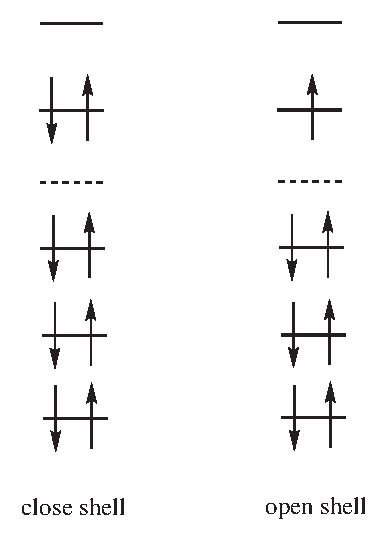
\includegraphics[scale=0.7]{rhfuhf.eps}
\caption{close shell and open shell} \label{SIC1}
\end{center}
\end{figure}

For each spatial orbital, it's only allowed maximumly $2$ electrons to reside
in. Such restriction is attributed from the Pauli principle that
there's no two electrons can share the same quantum states.
Therefore, complying with the energy minimization principle, that only
two electrons can be arranged into one orbital (such two electrons are
different in spin states).

For the quantum system which has single electron, where the number of
$\alpha$ electrons does not equal to the number of $\beta$ electrons,
the restriction above should be broken up. From the discussion of the
Hatree-Fock function, we can know that the spin is directly associated
with the total energy via the exchange effects. If the $\alpha$
electrons is more than the $\beta$ electrons, then it can be expected
that they are effected by different ``surroundings'' so that the total
energy for $\alpha$ electrons must be different with the total energy
for $\beta$ electrons. As a result, the sharing for the same spatial
orbital must be broken.

In this case, electrons in different spin states should be put into
independent spatial orbitals so that each of them forms some
independent partial orbital subspace:
\begin{equation}\label{}
\Psi =
 \begin{vmatrix}
   \varphi_{1}(1)\theta(1) &  \cdots & \varphi_{p}(1)\theta(1) & 
   \varphi_{p+1}(1)\theta(1) & \cdots  & \varphi_{n}(1)\theta(1)  \\
   \varphi_{1}(2)\theta(2) &  \cdots & \varphi_{p}(2)\theta(2) & 
   \varphi_{p+1}(2)\theta(2) & \cdots  & \varphi_{n}(2)\theta(2)  \\
   \cdots                  & \cdots  & \cdots                 & 
   \cdots                   & \cdots  & \cdots                  \\
   \varphi_{1}(n)\theta(n) & \cdots  & \varphi_{p}(n)\theta(n) & 
   \varphi_{p+1}(n)\theta(n) & \cdots  & \varphi_{n}(n)\theta(n)  \\
 \end{vmatrix}
\end{equation}
Here the $\theta(i)$ can be $\alpha(i)$ or $\beta(i)$, such method is
called unrestricted type of determinants.


%%%%%%%%%%%%%%%%%%%%%%%%%%%%%%%%%%%%%%%%%%%%%%%%%%%%%%%%%%%%%%%%%%%%%%%%%%%%%%%%%%%%%%%%%%
\section{Spin polarized states}
%
%  1  how to understand the spin polarized states
%  2  how to compose the approximated wave functions
%  3  some theorem that the alpha electrons and beta electrons
%     are forming some independent sets
%
In the above content, from the point of wave functions we have give
some general view about the spin phenomenon. In this section, we
will take another way to view the spin phenomenon in the chemistry.

In chemistry, it's very common to encounter the situation that the
characters of the given system is depending on the spin states. For
example, the characters of the radical systems etc. Here we can call
the quantum states used to describe such system as `` spin polarized
states'', which can be defined that the $\alpha$ electron density in
the given system does not equal to the $\beta$ electron density;
thus there exists some position of $\mathbf{r}$, where it has some
remaining spin:
\begin{equation}\label{}
\rho(\mathbf{r}) = \rho_{\alpha}(\mathbf{r}) -
\rho_{\beta}(\mathbf{r}) \neq 0
\end{equation}

Usually the density is expressed via the corresponding orbitals:
\begin{equation}\label{}
\rho_{\sigma}(\mathbf{r}) =
\sum_{i}|\varphi_{i\sigma}(\mathbf{r})|^{2}
\end{equation}
Where the $\sigma$ can be $\alpha$ or $\beta$. Then, the discussion
related to the spin states is attributed to the analysis on the
orbitals.

Basically there are two ways to compose the orbitals into the
approximate wave function for $n$ electrons system. One way is the
restricted method which is same as mentioned above. In this method
the $\alpha$ electrons and the $\beta$ electrons are forced into
pairs and each pair is stuffed into the orbital in the ascending
order of energy. Finally the unpaired electrons are arranged into
different orbitals. This method is also called ``restricted open
method''. The other way to compose the approximated wave function,
is the unrestricted way; that to let the $\alpha$ electrons and
$\beta$ electrons reside into different sets of orbitals, the
spatial part for the orbital for the different sets are independent
with each other.

Finally we wish to state some important distinguishment between such
two methods, is that the Slater determinant composed through the
unrestricted method is not the eigen states for the
$\hat{S}^{2}$. Hence in the post HF methods we usually do not use the
unrestricted method to compose the trial wave functions (Slater
determinant). the reason for this will be demonstrated in the next
section. 

%%%%%%%%%%%%%%%%%%%%%%%%%%%%%%%%%%%%%%%%%%%%%%%%%%%%%%%%%%%%%%%%%%%%%%%%%%%%%%%%%%%%%%%%%%
\section{General discussion for spin operators}
%
% 1  how to express the Sx, Sy, Sz
% 2  basic commutation rules on Sx, Sy, Sz
% 3  how to calculate the eigen value for the S^{2}
%    3.1  deal with Sz
%    3.2  deal with s_ and s+
%
%
for an arbitrary $n$ electrons system, we can define the spin
operator as:
\begin{equation}
  \hat{S}_{x} = \sum_{i=1}^{n}\hat{s}_{x}(i) \quad
  \hat{S}_{y} = \sum_{i=1}^{n}\hat{s}_{y}(i) \quad
  \hat{S}_{z} = \sum_{i=1}^{n}\hat{s}_{z}(i)
\end{equation}
Here each of $\hat{s}_{x}(i)$, $\hat{s}_{y}(i)$ or $\hat{s}_{z}(i)$
is working on the single particle wave function (where the ith
particle is residing in). Because we have assumed that there's no
correlation between the single particle wave functions, therefore
the total spin operator on each direction is simply the addition
between them.

Furthermore, the $\hat{S}_{x}$, $\hat{S}_{y}$ and $\hat{S}_{z}$
satisfy the basic commutation rules, which has been demonstrated in
the discussion of quantum mechanics:
\begin{align}\label{}
\hat{S}_{x}\hat{S}_{y} - \hat{S}_{y}\hat{S}_{x} &= i\hbar\hat{S}_{z}
\nonumber \\
\hat{S}_{y}\hat{S}_{z} - \hat{S}_{z}\hat{S}_{y} &= i\hbar\hat{S}_{x}
\nonumber \\
\hat{S}_{z}\hat{S}_{x} - \hat{S}_{x}\hat{S}_{z} &= i\hbar\hat{S}_{y}
\end{align}

Based on these basic spin operators, we can construct other useful
ones, namely the $\hat{S}^{2}$, $\hat{S}_{+}$ and $\hat{S}_{-}$:
\begin{equation}\label{}
\hat{S}^{2} = \hat{S}_{x}^{2} + \hat{S}_{y}^{2} + \hat{S}_{z}^{2}
\quad
\hat{S}_{+} = \hat{S}_{x} + i\hat{S}_{y} \quad
\hat{S}_{-}
=\hat{S}_{x} - i\hat{S}_{y}
\end{equation}

As what we have shown, usually in the quantum chemistry we choose
the $\hat{S}^{2}$ and $\hat{S}_{z}$ into the CSCCO, and the single
particle wave functions are always expressed as the eigen function
for the $\hat{S}_{z}$. Then for any composition based on the single
particle wave functions we can easily calculate the eigen values for
$\hat{S}_{z}$. However, how to calculate the eigen values for the
$\hat{S}^{2}$?

Here we only consider the determinants formed by the single particle
wave functions (however, it includes most of the cases in quantum
chemistry). To answer this question, we start from some relation
between the spin operators; which is easy to prove from the
definition:
\begin{equation}\label{}
\hat{S}^{2} = \hat{S}_{z}^{2} + \hat{S}_{z} + \hat{S}_{-}\hat{S}_{+}
\end{equation}

For the $\hat{S}_{z}$, to evaluate its eigen values is direct and
simple:
\begin{equation}\label{}
\left\{
  \begin{array}{ll}
    \hat{S}_{z}\alpha = \frac{1}{2} \\
    \hat{S}_{z}\beta  =-\frac{1}{2}
  \end{array}
\right.
\end{equation}
Thus for the determinant of $\Psi$, we can have:
\begin{align}\label{}
\hat{S}_{z}\Psi     &= \frac{1}{2}(n_{\alpha} - n_{\beta})\Psi
\nonumber
\\
\hat{S}_{z}^{2}\Psi &= \frac{1}{4}(n_{\alpha} - n_{\beta})^{2}\Psi
\end{align}

For the $\hat{S}_{-}$ and $\hat{S}_{+}$, it's a bit of complicated:
\begin{align}\label{}
\hat{S}_{-}\hat{S}_{+} &=
\sum_{i}\hat{s}_{-}(i)\sum_{j}\hat{s}_{+}(j)  \nonumber \\
&=\sum_{i}\hat{s}_{-}(i)\hat{s}_{+}(i) + \sum_{i \neq
j}\hat{s}_{-}(i)\hat{s}_{+}(j)
\end{align}

For the up operator and the down operator, from the basic
commutation relationship we can easily have the expressions below:
\begin{equation}\label{}
\left\{
  \begin{array}{ll}
    \hat{s}_{-}(i)\alpha(i) = \beta(i), &  \hat{s}_{-}(i)\beta(i) = 0 \\
    \hat{s}_{+}(i)\alpha(i) = 0       , &  \hat{s}_{+}(i)\beta(i) = \alpha(i) \\
  \end{array}
\right.
\end{equation}

For the determinant of $\Psi$, which can be written as:
\begin{equation}\label{}
\Psi =
\sum_{P}(-1)^{P}P(\varphi_{1}(1)\theta(1)\varphi_{2}(2)\theta(2)
\cdots\varphi_{n}(n)\theta(n))
\end{equation}

Since that the spin operator commutes with the permutation operator
of $P$, thus we can have:
\begin{multline}\label{}
\sum_{i}\hat{s}_{-}(i)\hat{s}_{+}(i)\Psi =
\sum_{P}(-1)^{P}P\Bigg\{\varphi_{1}(1)\varphi_{2}(2)
\cdots\varphi_{n}(n)
 \\
\sum_{i}\hat{s}_{-}(i)\hat{s}_{+}(i)
\Big(\theta(1)\theta(2)\cdots\theta(n)\Big)\Bigg\}
\end{multline}

In this expression, it's easy to see that only the $\beta$ electrons
can survive, thus we can have:
\begin{equation}\label{}
\sum_{i}\hat{s}_{-}(i)\hat{s}_{+}(i)\Psi = n_{\beta}\Psi
\end{equation}

On the other hand,  for the given $i$ and $j$; we have:
\begin{equation}\label{}
\begin{split}
\hat{s}_{-}(i)\hat{s}_{+}(j)\Psi &=
\sum_{P}(-1)^{P}P\Bigg\{\varphi_{1}(1)\varphi_{2}(2)
\cdots\varphi_{n}(n)
 \\
&\hat{s}_{-}(i)\hat{s}_{+}(j)
\Big(\theta(1)\cdots\alpha(i)\beta(j)\cdots\theta(n)\Big)\Bigg\} \\
    &=
\sum_{P}(-1)^{P}P\Bigg\{\varphi_{1}(1)\varphi_{2}(2)
\cdots\varphi_{n}(n)
 \\
&\Big(\theta(1)\cdots\beta(i)\alpha(j)\cdots\theta(n)\Big)\Bigg\} \\
\end{split}
\end{equation}

Therefore, the $\sum_{i \neq j}\hat{s}_{-}(i)\hat{s}_{+}(j)$ change
all the pairs of $\alpha(i)\beta(j)$ to be $\beta(i)\alpha(j)$, then
form new determinants. So we can abbreviate this operator as
$\sum_{i \neq j}\hat{P}_{ij}$.

All in all, we can have:
\begin{align}\label{SICeq:3}
\hat{S}^{2}\Psi &= \left(\frac{1}{4}(n_{\alpha} - n_{\beta})^{2} +
\frac{1}{2}(n_{\alpha} - n_{\beta}) + n_{\beta} + \sum_{i \neq
j}\hat{P}_{ij}\right)\Psi \nonumber \\
&=\left(\frac{1}{4}(n_{\alpha} - n_{\beta})^{2} +
\frac{1}{2}(n_{\alpha} + n_{\beta})\right)\Psi + \sum_{i \neq
j}\hat{P}_{ij}\Psi
\end{align}

Now take the $\Psi = |1s(1)\alpha(1)1s(2)\beta(2)2s(3)\alpha(3)|$ as
an example, to see that how to use the (\ref{SICeq:3}) to calculate
the eigen value for the $\hat{S}^{2}$:
\begin{equation}\label{}
\begin{split}
\hat{S}^{2}\Psi &= \left(\frac{1}{4}(2 - 1)^{2} + \frac{1}{2}(2 +
1)\right)|1s(1)\alpha(1)1s(2)\beta(2)2s(3)\alpha(3)| + \\
&|1s(1)\beta(1)1s(2)\alpha(2)2s(3)\alpha(3)| +
|1s(1)\alpha(1)1s(2)\alpha(2)2s(3)\beta(3)| \\
&=\frac{7}{4}|1s(1)\alpha(1)1s(2)\beta(2)2s(3)\alpha(3)| -
|1s(1)\alpha(1)1s(2)\beta(2)2s(3)\alpha(3)| \\
&=\left(\frac{1}{2}(\frac{1}{2} +
1)\right)|1s(1)\alpha(1)1s(2)\beta(2)2s(3)\alpha(3)|
\end{split}
\end{equation}
Thus, it's the eigen function for $\hat{S}^{2}$, and give the eigen
value of $3/4$.

Now finally let's give some illustration about some important concept
that why the unrestricted determinant is not the eigen function for
$\hat{S}^{2}$; this can be made clear through the definition of
$\hat{S}^{2}$ in (\ref{SICeq:3}). 

Take $|1s(1)\alpha(1)1s^{'}(2)\beta(2)|$ as an example. This
determinant gives $S_{z} = 0$, and it can be used to portray the
ground state for hydrogen gas ($H_{2}$). By the definition of
$\hat{S}^{2}$ in (\ref{SICeq:3}), we can have:
\begin{equation}
  \begin{split}
    \hat{S}^{2} |1s(1)\alpha(1)1s^{'}(2)\beta(2)| &= \left( 0 +
      1\right)|1s(1)\alpha(1)1s^{'}(2)\beta(2)| + \\
    & |1s(1)\beta(1)1s^{'}(2)\alpha(2)| \\
&=  |1s(1)\alpha(1)1s^{'}(2)\beta(2)| +
    |1s(1)\beta(1)1s^{'}(2)\alpha(2)|
  \end{split}
\end{equation}
Compared with the former example for
$|1s(1)\alpha(1)1s(2)\beta(2)2s(3)\alpha(3)|$, here the
distinction is that in the second determinant of
$|1s(1)\beta(1)1s^{'}(2)\alpha(2)|$; if we exchange the electron label
between $1$ and $2$, we will get $|1s^{'}(1)\alpha(1)1s(2)\beta(2)|$,
which is obviously different from the first one. Hence the inequality
of the partial part of MO lead to the determinants unable to cancel
with each other. That's why the unrestricted type of determinants are
no longer to be the eigen states for the $\hat{S}^{2}$. 



%%%%%%%%%%%%%%%%%%%%%%%%%%%%%%%%%%%%%%%%%%%%%%%%%%%%%%%%%%%%%%%%%%%%%%%%%%%%%%%%%%%%%%%%%%
\section{How to form the spin adapted configurations}
%
%
%  in this part, we discuss that how to form the
%  spin adapted configurations
%  1   general strategy
%  2   discuss the singlet, doublet and triplet.
%      the eigen states and eigen values
%  3   extend the idea to arbitrary sin states
%
%
Now based on the discussion above, let's talk about that how to form
the spin adapted configurations; which is one of important step in
CI and it's derivative methods.

Basically, the spin adapted configurations in the trial wave
functions can be achieved by the following two steps:
\begin{itemize}
  \item Selecting orbitals to form the Slater determinants.
  From the result of Hatree-Fock calculation, we can select
  a group of orbitals to form the determinants. Here the
  Slater determinants should be only formed in restricted way
  because only this kind of determinants can be the eigen states for
  the $\hat{S}^{2}$ and $\hat{S}_{z}$.
\item After the first step, the determinants will be combined into
  some linear combination so that it's the eigen states for the
  $\hat{S}^{2}$ and $\hat{S}_{z}$. Here we may apply some techniques to
  do so, for example to use the project operator to ``sort out'' the
  Slater determinants we want. Finally, we can get the so called
  ``spin adapted configurations''. According to the rules introduced
  above, the spin adapted configurations which give different eigen
  values for the $\hat{S}^{2}$ or $\hat{S}_{z}$ will not mixing with
  each other, so the Hamiltonian matrix will be shaped into blocks.
\end{itemize}

Next, we wish to present several examples to show how to construct
the spin adapted configurations. In the discussion below the general
form of determinants will be considered ($n$ electrons are arranged
into $m$ orbitals):
\begin{equation}\label{}
\Psi = |\varphi_{1}(1)\theta(1)\cdots\varphi_{m}(n)\theta(n)|
\end{equation}

the most simplest eigen state for the spin operator of $\hat{S}^{2}$
and $\hat{S}_{z}$ is the singlet, which can be defined as:
\begin{equation}\label{SICeq:4}
\left\{
  \begin{array}{ll}
    \hat{S}_{z}\Psi = 0 \Rightarrow S = \max(S_{z}) = 0\\
    \hat{S}^{2}\Psi = S(S+1) = 0
  \end{array}
\right.
\end{equation}
Here, for a certain $S$ there will be $2\max(S_{z}) + 1$ degenerate
states, they are different in $S_{z}$; thus we can see that there's
only one eigen state satisfy the (\ref{SICeq:4}); so we call this
state as ``singlet''.

It's easy to see that only the close shell determinant can be the
singlet (see the figure of \ref{SIC2}). In the open shell case, we
can reverse the spin on Z direction for the unpaired electrons so
that to form the determinants which have different $S_{z}$ value.
but they can also correspond to same $\hat{S}$. Therefore, there are
more than one determinants corresponding to the $\hat{S}$ so that the
open shell determinants can not correspond to the singlet.
\begin{figure}
\begin{center}
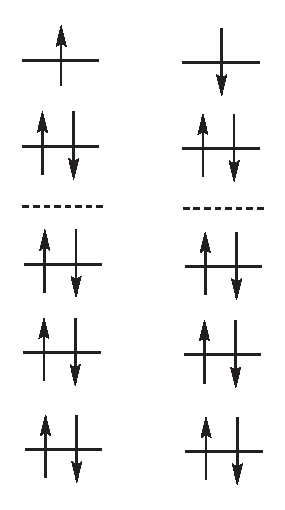
\includegraphics[scale=0.7]{spin_chem_1.eps}
\caption{doublet states} \label{SIC2}
\end{center}
\end{figure}

Similarly we can define the ``doublet'' states, which is:
\begin{equation}\label{SICeq:5}
\left\{
  \begin{array}{ll}
    \hat{S}_{z}\Psi = \frac{1}{2}, -\frac{1}{2}
    \Rightarrow S = \max(S_{z}) = \frac{1}{2}\\
    \hat{S}^{2}\Psi = S(S+1) = \frac{3}{4}
  \end{array}
\right.
\end{equation}
It's called doublet because for a certain $S$ it has two degenerate
states, one gives the eigen value of $1/2$ for $\hat{S}_{z}$, the
other gives $-1/2$. Such determinants are pictured in (\ref{SIC2}).

Moreover, we can see that the doublet can only be the determinants
shown in figure of (\ref{SIC2}). If there are more than two orbitals
having the single electron residing on, we can see that the maximum
of $S_{z}$ must exceed or equal to $1$ ($\max(S_{z}) \leq 2*1/2 =
1$), thus there will be at least $3$ eigen states for the
$\hat{S}_{z}$, so it's not the doublet.

On the other hand, we can use the $\hat{S}^{2}$ defined in
(\ref{SICeq:3}) to prove that each of the determinant is the eigen
state for $\hat{S}^{2}$. For the doublet, we can generally assume
the single electron residing on its highest orbital:
\begin{align}\label{SICeq:6}
\Psi &= |\varphi_{1}(1)\alpha(1)\varphi_{1}(2)\beta(2) \cdots
\nonumber \\
&\varphi_{m-1}(n-1)\alpha(n-1)\varphi_{m-1}(n-1)\beta(n-1)
\varphi_{m}(n)\theta(n)|
\end{align}
Here the $\theta(n)$ can be $\alpha$ or $\beta$.

In the expression of the $\hat{S}^{2}$, we can see that operator of
$\sum_{i \neq j}\hat{P}_{ij}$ should only change the pair of
electrons which share the same orbitals, else there will be pair of
electrons with same spin states on the same orbital, it will be
zero. So we can have (here below the total number of electrons are
$2n+1$):
\begin{equation}\label{}
\begin{split}
\hat{S}^{2}\Psi &= \left(\frac{1}{4} + \frac{1}{2}(2n +
1)\right)\Psi + n|\varphi_{1}(1)\alpha(1)\varphi_{1}(2)\beta(2)
\cdots  \\
&\varphi_{i}(k)\beta(k)\varphi_{i}(k+1)\alpha(k+1)\cdots
\varphi_{m}(n)\theta(n)| \\
&=\frac{3}{4}\Psi + n\Psi -n\Psi \\
&=\left(\frac{1}{2}(\frac{1}{2} + 1)\right)\Psi
\end{split}
\end{equation}

Next, we can discuss the ``triplet'', which is defined as:
\begin{equation}\label{SICeq:7}
\left\{
  \begin{array}{ll}
    \hat{S}_{z}\Psi = 1, 0,  -1
    \Rightarrow S = \max(S_{z}) = 1\\
    \hat{S}^{2}\Psi = S(S+1) = 2
  \end{array}
\right.
\end{equation}
Thus for the $S=1$ there are three eigen states corresponding to
different $S_{z}$ values. Similar with the discussion for singlet
and doublet, we can see that the triplet state should has two single
electron orbitals, which can be pictured in the figure of
(\ref{SIC3}).
\begin{figure}
\begin{center}
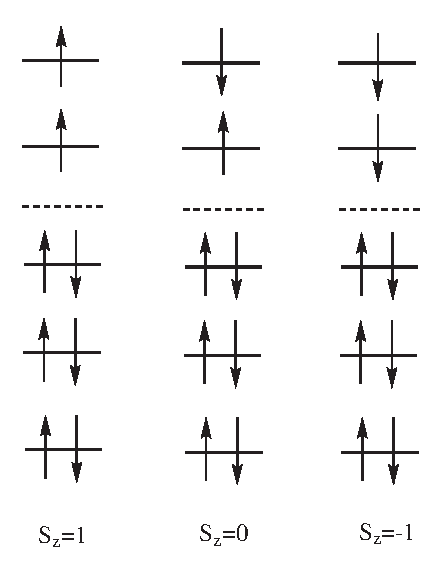
\includegraphics[scale=0.7]{triplet.eps}
\caption{how to form a triplet} \label{SIC3}
\end{center}
\end{figure}

Now we derive the expression of the triplet eigen states for both of
the $\hat{S}^{2}$ and $\hat{S}_{z}$. It's assumed that the
determinants has such form:
\begin{equation}\label{}
\Psi = |\varphi_{1}(1)\alpha(1)\varphi_{1}(2)\beta(2) \cdots
\varphi_{m-1}(n-1)\theta(n-1) \varphi_{m}(n)\theta^{'}(n)|
\end{equation}
Here the $\theta$ and $\theta^{'}$ can be $\alpha$ or $\beta$.

Firstly we note that this case is different form the singlet and
doublet, where all the eigen states for the $\hat{S}^{2}$ and
$\hat{S}_{z}$ are non-degenerate; here the $\hat{S}_{z}$ has two
degenerate eigen states, they all give $S_{z} = 0$:
\begin{equation}\label{}
\Psi_{01} = |\varphi_{1}(1)\alpha(1)\varphi_{1}(2)\beta(2) \cdots
\varphi_{m-1}(n-1)\alpha(n-1) \varphi_{m}(n)\beta(n)|
\end{equation}
\begin{equation}\label{}
\Psi_{02} = |\varphi_{1}(1)\alpha(1)\varphi_{1}(2)\beta(2) \cdots
\varphi_{m-1}(n-1)\beta(n-1) \varphi_{m}(n)\alpha(n)|
\end{equation}
Therefore, for the $S_{z} = 0$, the eigen state of the $\hat{S}^{2}$
must be the linear combination between the two determinants. By
using the $\hat{S}^{2}$ defined in (\ref{SICeq:3}), we can finally
have:
\begin{equation}\label{}
\Psi_{0} = \frac{1}{\sqrt{2}}(\Psi_{01} + \Psi_{02})
\end{equation}

On the other hand, for the $S_{z} = 1$ and $S_{z} = -1$, the eigen
states are non-degenerate:
\begin{equation}\label{}
\Psi_{1} = |\varphi_{1}(1)\alpha(1)\varphi_{1}(2)\beta(2) \cdots
\varphi_{m-1}(n-1)\alpha(n-1) \varphi_{m}(n)\alpha(n)|
\end{equation}
\begin{equation}\label{}
\Psi_{-1} = |\varphi_{1}(1)\alpha(1)\varphi_{1}(2)\beta(2) \cdots
\varphi_{m-1}(n-1)\beta(n-1) \varphi_{m}(n)\beta(n)|
\end{equation}
Thus they must be the eigen states for the $\hat{S}^{2}$. By using
the expression in (\ref{SICeq:3}), we can also prove this point.

From the three examples above we can extend the idea to the
arbitrary spin states. For some spin state of $\Psi$ where the
spatial orbitals are fixed, we can construct a lot of eigen states
for $\hat{S}_{z}$, and some may be degenerate. For these degenerate
states the eigen state for the $\hat{S}^{2}$ must be linear
combination of them. For deriving the eigen states for both of the
$\hat{S}_{z}$ and $\hat{S}^{2}$, it has been developed many
effective methods such as the ``Young Picture''
method\cite{aoqingTang}. The reader can refer to such materials for
more help.


%%%%%%%%%%%%%%%%%%%%%%%%%%%%%%%%%%%%%%%%%%%%%%%%%%%%%%%%%%%%%%%%%%%%%%%%%%%%%%%%%%%%%%%%%%
\section{Spin contamination}
%
% 1  give the general expression for the unrestricted wave function
% 2  why the states are mixed together
% 3  the reason for the spin contamination
% 4  how to reduce the spin contamination
%
The unrestricted type of wave functions usually have the spin
contamination problem. This problem is attributed from the mixture
of other spin states.

For the general unrestricted wave function of $\Psi$, the general
expression is below (we suggest that we have $k$ $\alpha$ electrons
and $l=n-k$ $\beta$ electrons):
\begin{equation}\label{}
\Psi =
 \begin{vmatrix}
   \varphi_{1}(1)\theta(1) &  \cdots & \varphi_{p}(1)\theta(1) & 
   \varphi_{p+1}(1)\theta(1) & \cdots  & \varphi_{n}(1)\theta(1)  \\
   \varphi_{1}(2)\theta(2) &  \cdots & \varphi_{p}(2)\theta(2) & 
   \varphi_{p+1}(2)\theta(2) & \cdots  & \varphi_{n}(2)\theta(2)  \\
   \cdots                  & \cdots  & \cdots                 & 
   \cdots                   & \cdots  & \cdots                  \\
   \varphi_{1}(n)\theta(n) & \cdots  & \varphi_{p}(n)\theta(n) & 
   \varphi_{p+1}(n)\theta(n) & \cdots  & \varphi_{n}(n)\theta(n)  \\
 \end{vmatrix}
\end{equation}

Commonly we do not require that the spatial part of orbital for
$\alpha$ electron and $\beta$ electron should be same, because
they varies independently. In such circumstance, the wave function
is the eigen state for the $\hat{S}_{z}$, because it gives certain
eigen value for the $\hat{S}_{z}$ ($S_{z} = \frac{1}{2}(k-l)$).
However, such wave function is usually not the eigen function for
the $\hat{S}^{2}$, which is just as what we have demonstrated.

From the spin discussion in quantum mechanics, we know that for the
eigen states with some certain $S_{z}$ (e.g. $S_{z} = 1$); there may
exist many states corresponding to it, they come from the eigen
states with different $S$ eigen value (for example, as $S_{z} = 1$,
it has eigen states coming from $S=1,2,3 \cdots$).

According to such analysis, we can have the general principle below;
that the unrestricted wave function of $\Psi$ with $S_{z} = m$, can
be composed by the eigen states whose $S_{z} = m$, but their $S =
m+2, m+4, m+6, \cdots$ etc.:
\begin{align}\label{}
\Psi_{siglet} &= c_{1}\ket{1} + c_{2}\ket{3} + c_{3}\ket{5} + \cdots
\nonumber \\
\Psi_{doublet} &= c_{1}\ket{2} + c_{2}\ket{4} + c_{3}\ket{6} +
\cdots
\nonumber \\
\Psi_{triplet} &= c_{1}\ket{3} + c_{2}\ket{5} + c_{3}\ket{7} +
\cdots
\end{align}

Here we have some question that for the $\Psi$ with $S_{z} = m$, why
the $m+1$, $m+3$ states etc. do not contribute to it?

To answer this question, we have to remember that for the state with a
certain $S$ value, it only has one eigen state that $S_{z} = m$.  If
the spatial part of the determinants are fixed, and we require that it
gives certain $S$ value; since $S = \max (S_{z})$, and the number of
single electrons in the determinant is $2\max (S_{z})$; hence the
number of single electrons are $2S$. 

In this case, the higher spin state with different $S$ value should be
those that ``fire up'' the electrons from the occupied orbitals to the
virtual orbitals so as to produce new single electrons in this
determinant. In this process, the action will always generate two new
single electron orbital, thus the higher spin states should increase
by degrees by $2$ (obviously this value is related to the $S$
according to the analysis above).

Based on the analysis above, we can know that the spin contamination
is some inherent character for the unrestricted wave functions.
Traditionally in quantum chemistry, there has been developed many
ways to reduce the spin contamination, such as the use of
``annihilate operator'' to project the right component of the spin
state from the mixtures. For further study, the reader may also
refer to the book given by Tang\cite{aoqingTang}.

%%%%%%%%%%%%%%%%%%%%%%%%%%%%%%%%%%%%%%%%%%%%%%%%%%%%%%%%%%%%%%%%%%%%%%%%%%%%%%%%%%%%%%%%%%


%%% Local Variables: 
%%% mode: latex
%%% TeX-master: "../../main"
%%% End: 
